
\chapter{Systémový manuál}

Tento manuál slúži pre popísanie crawlera na úrovni vhodnej pre úpravu systému a rozširovanie jeho funkcionalít. 

% Scala je vysoko úrovňoví jazyk schopný lepšej reprezentácie abstrakcie ako diagramy a bežná ľudská reč. Táto dokumentácie je určená primárne pre programátora so znalosťou tohto jazyka, preto popisuje len zodpovednosti modulov. 

\section{Moduly}
V tejto podkapitole popíšeme stručne zodpovednosť modulov a ich rozhranie voči zvyšku systému. 

\subsection{UrlManager}
Modul zodpovedný za ukladanie stavu crawlovania a jeho perzistovanie. Hlavná implementácia využíva jednoduché dátové štruktúry - zoznam a množinu na ukladanie stavu na perzistovanie uskutočnuje serializáciou na disk. Ak crawler má bežať nepretržite dni, je potrená nová implementácia. Perzistovanie iba incrementov, nie celého stavu alebo prejdenie k využitiu relačnej databázy. Tej sa chceme ale vyhnúť pre zachovanie jednoduchosti infraštruktúry. Jej rozhranie a implementácie sú znázornené na diagrame tried \ref{o:urlManChart}. 

\begin{figure}[!ht]
    \centering
    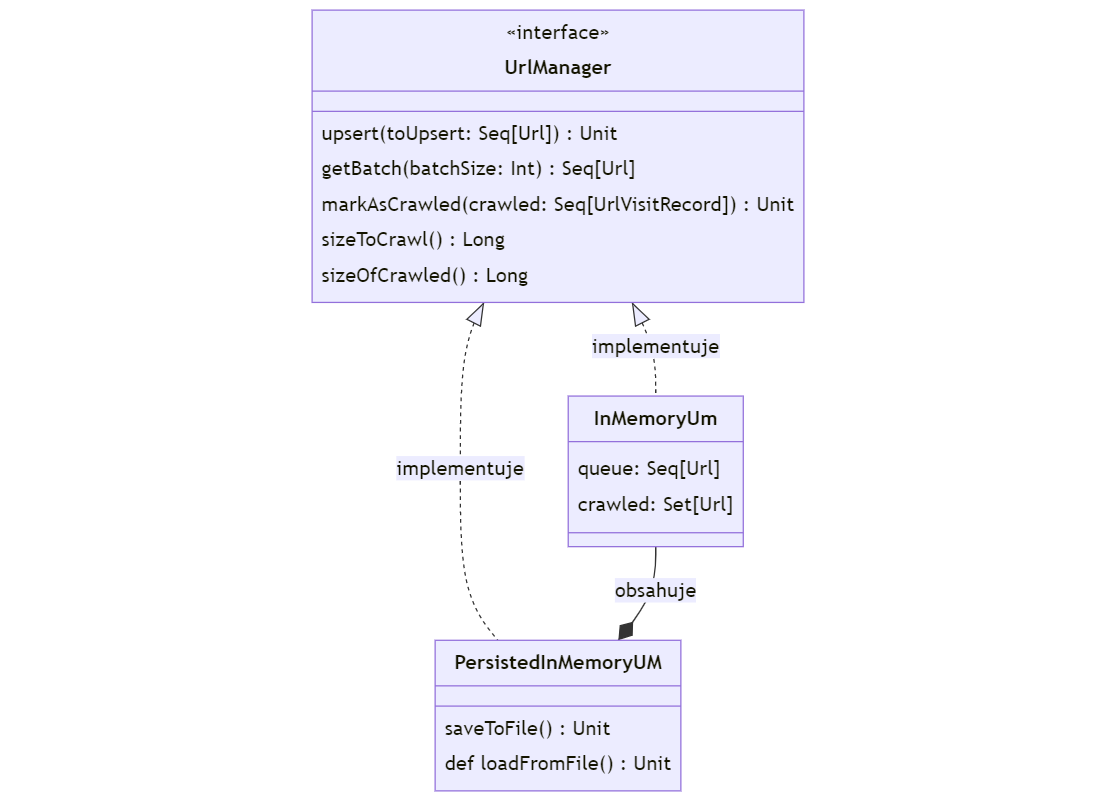
\includegraphics[width=1\textwidth]{figures/urlManagerChart.png}
    \caption{Diagram tried UrlManager\label{o:urlManChart}}
\end{figure}


\subsection{Repository}
Modul zodpovedný za ukladanie výsledkov. Vytvorené implementácie sú ukladanie do jedného CSV súboru, teda pridávanie výsledkov na jeho koniec. A ukladanie každého kroku do samostatného CSV súboru. Taktiež sme vytvorili implementáciu, ukladajúcu výsledky do pamäte. Tá je určenú len na testovanie zvyšných modulov. Jej rozhranie a implementácie sú znázornené na diagrame tried \ref{o:repoClassChart}. 

\begin{figure}[!ht]
    \centering
    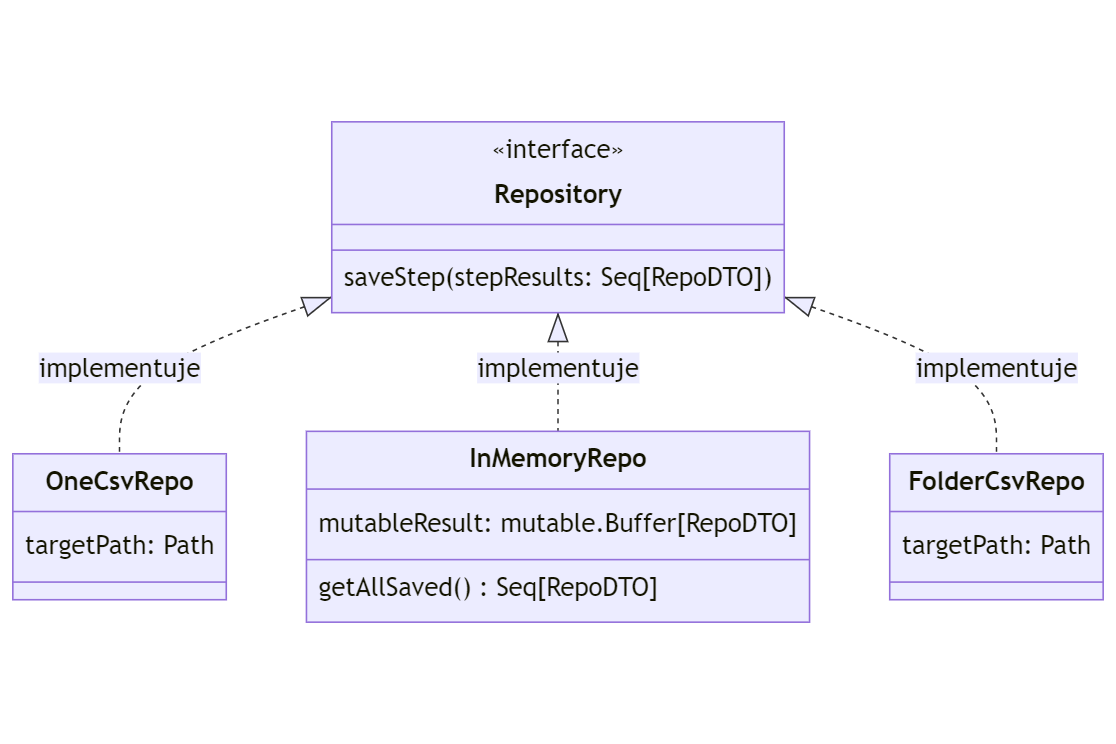
\includegraphics[width=1\textwidth]{figures/repositoryClassChart.png}
    \caption{Diagram tried Repository\label{o:repoClassChart}}
\end{figure}

\subsection{Modul crawlovania}
Nejde o samostatnú triedu ale o sadu funkcii, jedna volajúca druhú druhú. Je to jediné miesto paralelizácie a je striktne separované od zvyšku systému. Teda zvyšné moduly vôbec nevedia o paralelizácii a nemusia sa tomu prispôsobovať. Jeho úlohou je pre každú pridelenú adresu vrátiť CrawlResult. Na extrahovanie dát z HTML dokumentu a rozhodnutia či nájdená adresa je v prehľadávanej doméne využíva modul Extraktor. \todo{flow diagram volania tried}

\subsection{Extraktor}
V kóde je nazvaný DomainScraper. Slúži extrahovanie obsahu z HTML dokumentu a na určenie či adresa patrí pod jeho doménu. Každá implementácia je zameraná na jednu doménu. Pre pridanie novej domény na extrakciu je potrebné implementovať interface DomainScraper a pridať ho do zoznamu v objekte (scala alternatíva k java singletonu) SupportedDomains. Pre uľahčenie inicializácie crawlera navrhujeme v budúcnosti nastavovanie SupportedDomains cez CrawlerContext. Pre výber správneho extraktora pre spracovávanú adresú slúži DomainFilter s metódou getDomainScraper. Vzťahy medzi týmito triedami sú vyjadrené diagramom \ref{o:domScraperChart}.

\begin{figure}[!ht]
    \centering
    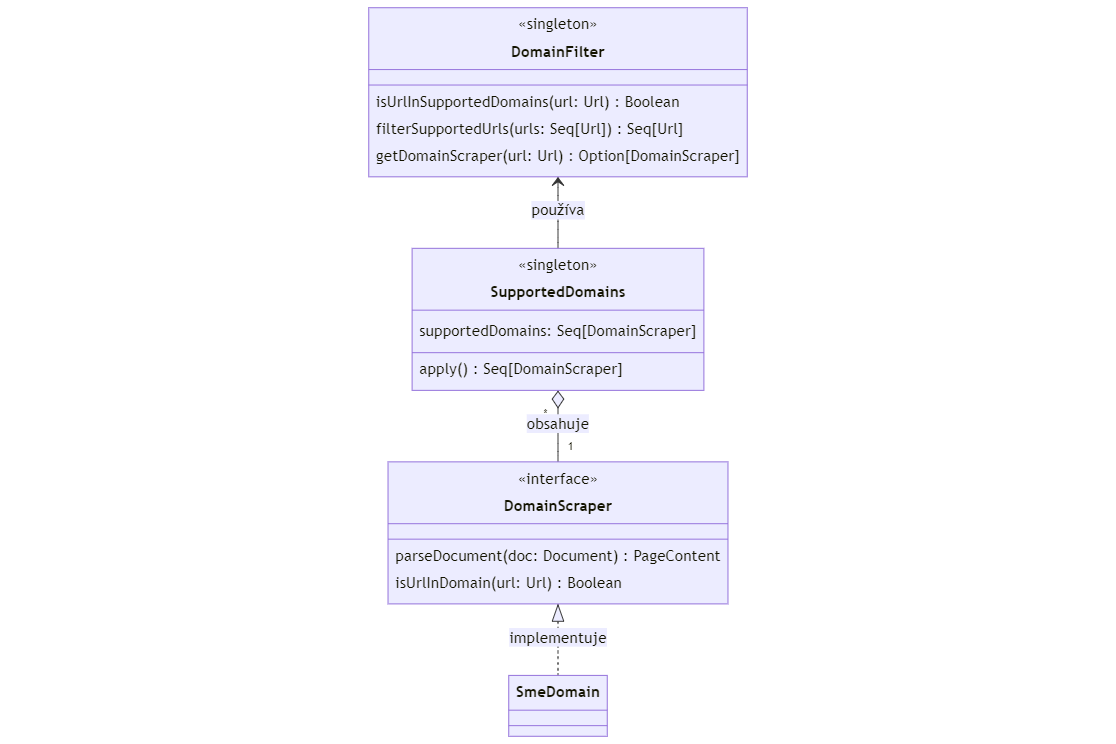
\includegraphics[width=1\textwidth]{figures/domainScraperChart.png}
    \caption{Diagram tried Extraktora\label{o:domScraperChart}}
\end{figure}

\subsection{Koordinátor}
Je to hlavná časť programu, sprostredkúvajúca komunikáciu medzi modulmi. V kóde je implementovaný ako trieda MyCrawler. 




\section{Pomocné triedy}
V programe používame triedy, ktoré nemôžeme považovať za samostatné moduly. V tejto podkapitole popíšeme stručne ich zodpovednosťa ich rozhranie voči zvyšku systému. 

\subsection{CrawlerContext}
Je to trieda slúžiaca na injektovanie závislostí crawleru. Teda aby sme mohli pri inicializácii crawlera určiť aké implementácie modulov chceme použiť a tým jednoducho meniť jeho správanie. Napríklad pri integračných testoch používať testovacie implementácie. Jeho štruktúru môžeme vidieť na diagrame tried \ref{o:classDiagramContextManual}.

\begin{figure}[!ht]
    \centering
    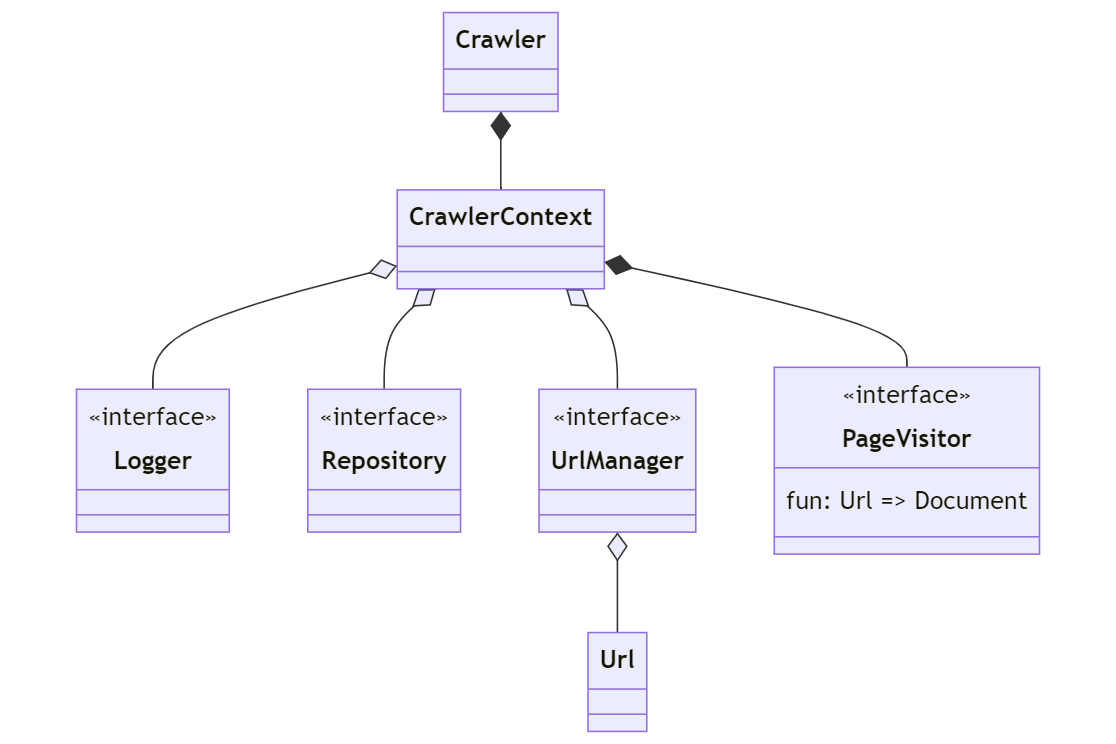
\includegraphics[width=1\textwidth]{figures/classDiagramContext.png}
    \caption{Diagram tried CrawlerContext\label{o:classDiagramContextManual}}
\end{figure}


\subsection{Logger}
Pomocný modul, slúžiaci na robenie záznamov o behu programu. Oproti bežnej implementácii umožňuje meranie trvania operácii. Napríklad ako dlho trvá zápis výsledkov. Takto vieme monitorovať priebeh crawlovania, čo je nápomocné pre jeho optimalizáciu a odhaľovanie chýb. \todo{Mozno class diagram ak bude malo miesta}



\section{Beh programu a paralelizácia}
Beh programu sme rozdelili do krokov. To nám umožnilo úplnú separáciu paralelného výpočtu od zvyšných modulov. Tým sme docielili, že iné moduly nemusia riešiť paralelizačnú logiku. Jeden krok je vyjadrený pomocou sekvenčného diagramu \ref{o:seqStepManual}.

\begin{figure}[!ht]
    \centering
    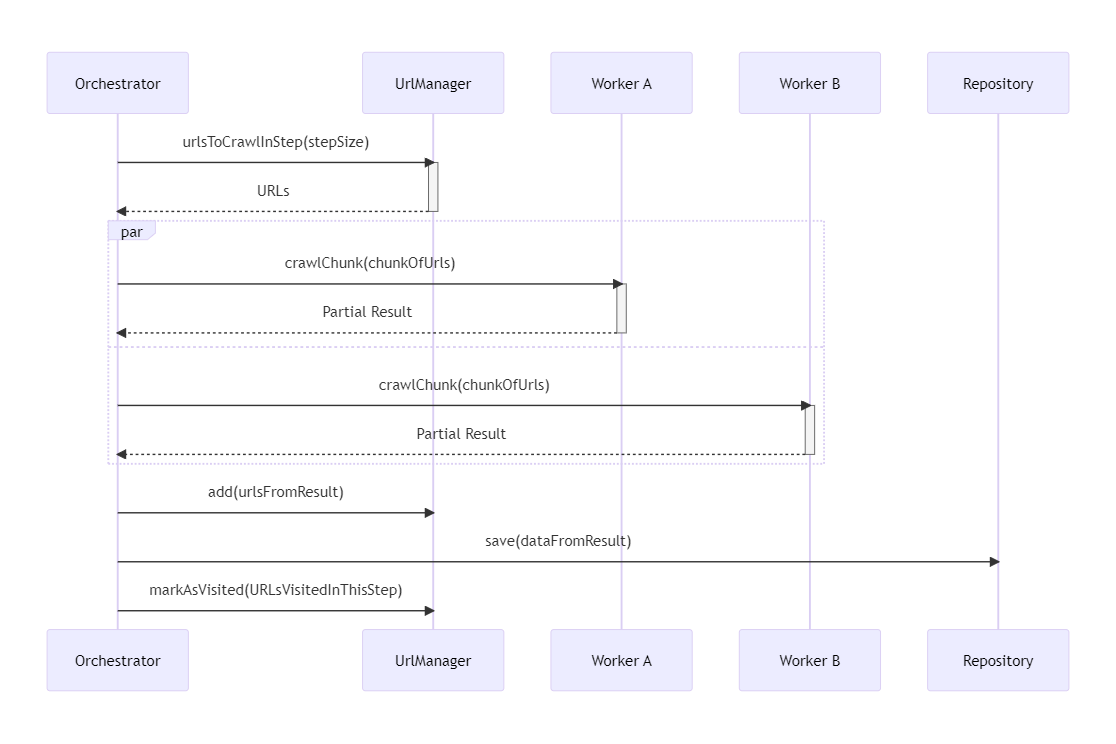
\includegraphics[width=1\textwidth]{figures/seqDiagCrawlStep.png}
    \caption{Sekvenčný diagram jedného kroku\label{o:seqStepManual}}
\end{figure}

